%!TEX root = ../report.tex
\chapter{Introduction}
\label{ch:context}
This document depicts the software architecture of Home Energy Monitoring System as the first assignment of Software Patterns course. We proclaim ourself as a software architect team working on the Home Energy Monitoring System (HEMS).

Energy is one of main concern in household. The problem is, how to monitor energy usage of a particular house in order to prevent useless consumption of energy and even how to save energy, resulting in lower household expenses for energy cost. This system focuses on electricity, as one of the main energy consumption of a house.

This system allows the user to collect and store their electricity consumption. This system will also have a web dashboard that shows the graph of electricity consumption, which user can adjust the time range of the graph to see different data, and other useful data such as which device uses the electricity the most, etc. The data, which will be stored in our database, will be used to do analysis that will help user to predict their upcoming electricity bill in the next month and other required analysis. This system also provide a fault-tolerant computing platform to compute this analysis.

The data collection is not our part, we leave this portion of the system to the third party developers. Basically, we provide a cloud computing environment (SaaS) to do energy management system. Everyone can join this system through provided API.

\section{System Context} % (fold)
\label{sec:system_context}
This system provides monitoring for more than one house. Many houses can connect to the system through Internet. Sensors will be located at every device that users are willing to monitor. Real time measurement of electricity consumption will be sent to the HEMS server via Internet protocol by the sensor. Figure \ref{fig:system-context} shows the system context of the HEMS.

\begin{figure}[!ht]
	\centering
	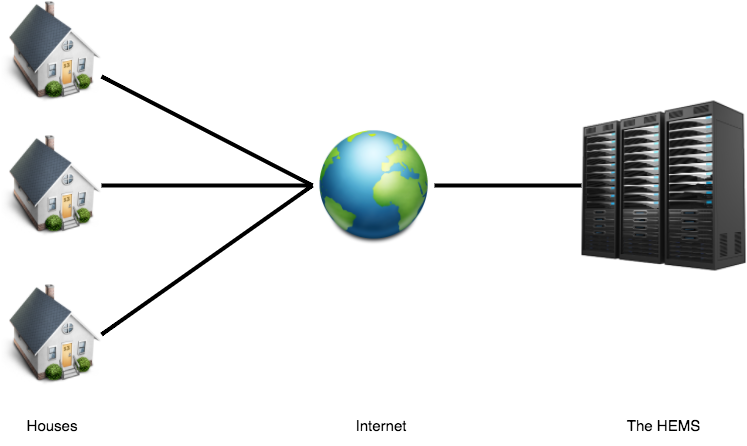
\includegraphics[width=0.7\textwidth]{1-context/images/SP-system-context.png}
	\caption{The HEMS system context.}
	\label{fig:system-context}
\end{figure}

As the sensors send the electricity measurement, no servers or any computing devices are needed to be installed in each house. This will make this system to be simple and easy to be implemented in each house. Users may see the energy consumption through the web dashboard via computers, tablets, smartphones, or any devices that are able to connect to the Internet. They may also place a TV or a screen in their house so that everyone in the house can see their energy consumption.